\documentclass{beamer}
\usepackage[utf8]{inputenc}
\usepackage[T1]{fontenc}
\usepackage[english]{babel}
\usepackage{graphicx}
\usepackage{times}

\usetheme{AGH}

\title[Technologie mobilne]{Broadcast receivers, content providers, services, async tasks}

\author[M. Nowotyński, M.Moskal, K. Osuch]{Mateusz Nowotyński \and Marcin Moskal \and Kamil Osuch}

\date[12.12.2017]{12.12.2017}

%\setbeamertemplate{itemize item}{\textbullet}

\begin{document}

{
%\usebackgroundtemplate{
\includegraphics[width=\paperwidth]{titlepage}} % wersja angielska
\usebackgroundtemplate{
\includegraphics[width=\paperwidth]{titlepagepl}} % wersja polska
 \begin{frame}
   \titlepage
 \end{frame}
}

%---------------------------------------------------------------------------


\begin{frame}{Broadcast Receivers}

\begin{block}{Do czego to służy?}
	BroadcastReceiver pozwala nam na odbieranie powiadomień (Systemu bądź innej aplikacji) wewnątrz naszej aplikacji. Takim powiadomieniem może być na przykład informacja o nowej wiadomości SMS bądź rozładowanej baterii.
\end{block}
\end{frame}


\begin{frame}{Tworzenie Broadcast Receiver'a}
	Żeby zbudować nasz własny BroadcastReceiver musimy wykonać dwie czynności:
	\begin{enumerate}
		\item Stworzyć podklasę klasy BroadcastReceiver
		\item Wyspecyfikować receiver w manifeście aplikacji lub bezpośrednio w kodzie
	\end{enumerate}
\end{frame}


\begin{frame}{Przykład klasy Broadcast Receiver'a}
	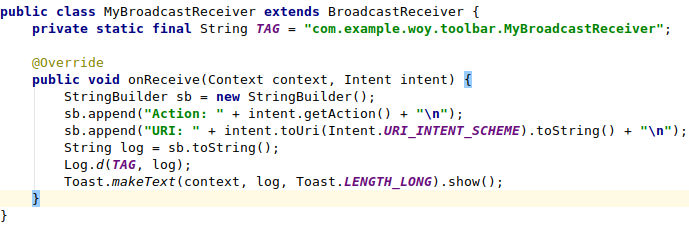
\includegraphics[width=\textwidth]{receiver}
\end{frame}


\begin{frame}{Dodanie do manifestu}
	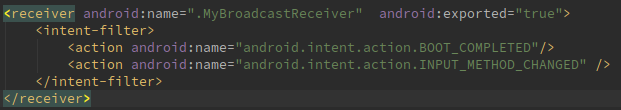
\includegraphics[width=\textwidth]{manifest}
	\begin{block}{Uwaga!}
		Powyższe rozwiązanie nie zadziała w wersji API wyższej niż 25. Nie można wtedy użyć manifestu do zadeklarowania receiver'a dla większości implicit broadcast'ów (z wyjątkiem kilku wyszczególnionych).
	\end{block}
\end{frame}

\begin{frame}{Rejestracja w kodzie}
	\centering
	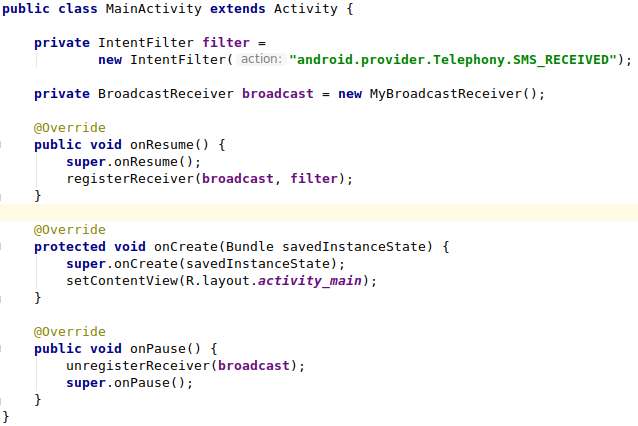
\includegraphics[height=0.7\textheight]{code-registration}
\end{frame}

\begin{frame}{Rejestracja - kontekst}
	\begin{block}{Manifest}
		W przypadku dodania deklaracji receiver'a do manifestu, jest on rejestrowany w momencie zainstalowania aplikacji. Receiver staje się wtedy oddzielnym punktem wejścia aplikacji. Oznacza to, że system może wystartować aplikację i przekazać wysyłany broadcast do receiver'a.
	\end{block}
	\begin{block}{Rejestracja w kodzie}
		Receiver'y zarejestrowane w kodzie odbierają broadcast'y tak długo jak kontekst w którym zostały zarejestrowane jest aktywny.
	\end{block}
\end{frame}

\begin{frame}{Wysyłanie broadcast'ów}
	Android oferuje trzy sposoby wysyłania broadcastów:
	\begin{itemize}
		\item<1-> \textbf{sendOrderedBroadcast} - wysyła broadcast do jednego receiver'a na raz. Gdy receiver zakończy 	swoje wykonanie, może propagowac rezultat do innego receiver'a, lub też całkowicie przerwać broadcast.	Kolejność broadcastów może być określana za pomocą atrybutu \textbf{android-priority}
		\item<2-> \textbf{sendBroadcast} - tzw. normalny broadcast, wysyła broadcast do wszystkich receiver'ów w nieokreślonej kolejności. Jest szybszy, ale nie można kontrolować przeplywu broadcast'u między receiver'ami, czy go zatrzymać.
		\item<3-> \textbf{LocalBroadcastManager.sendBroadcast} - wysyła broadcast do receiver'ów, które są w tej samej aplikacji, co strona wysyłająca. 
	\end{itemize}
\end{frame}

\begin{frame}{Przykład wysyłania broadcast'ów}
	\centering
	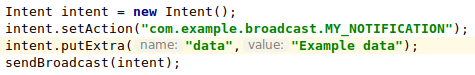
\includegraphics[width=\textwidth]{send-broadcast}
	\begin{block}{Uwaga!}
		Pomimo tego, że Intent jest używany zarówno do wysyłania broadcast'ów, jak i startowania activity (przy pomocy \textbf{startActivity}), akcje te nie są ze sobą powiązane. Broadcast receiver'y nie odbiorą akcji używanej do wystartowania activity.
	\end{block}
\end{frame}

\begin{frame}{Ograniczenia broadcast'ów - uprawnienia}
	\begin{block}{Wysyłanie}
		\textbf{sendBroadcast(intent, permission)} - wysłany w ten sposób broadcast może zostać odebrany tylko przez receiver posiadający uprawnienie \textbf{permission} 
	\end{block}
	\begin{block}{Odbieranie}
		\textbf{registerBroadcaster(receiver, intent-filter, permission, handler)} - Receiver odbierze broadcast'y tylko od wysyłających, którzy posiadają uprawnienie \textbf{permission}
	\end{block}
\end{frame}

%Content providers

\begin{frame}{Content providers}
	\begin{block}{}
		Content provider pomaga aplikacji w zarządzaniu dostępem do danych przechowywanych przez samą siebie czy inne aplikacje, i udostępnia sposób na dzielenie się danymi z innymi aplikacjami. 
	\end{block}
	\begin{block}{}
		Content provider prezentuje dane zewnętrznym aplikacjom jako jedna lub wiele tabel, które są podobne do tabel z relacyjnych baz danych. Wiersz reprezentuje instancję jakiegoś typu danych, który gromadzi w sobie provider. Kolumna reprezentuje indywidualną część danych dla konkretnej instancji.
	\end{block}
\end{frame}

\begin{frame}{Dostęp do danych}
	\begin{block}{}
		Do uzyskania dostępu do danych wykorzystywany jest \textbf{ContentResolver}. Każdy kontekst aplikacji przechowuje instancję klasy ContentResolver, do której dostęp obywa się poprzez metodę \textbf{getContentResolver()}. 
	\end{block}
	\begin{block}{Metody operujące na danych}
		Metody klasy ContentResolver udostępniają podstawowe operacje CRUD(create - \textbf{insert()}, read - \textbf{query()}, update - \textbf{update()}, delete - \textbf{delete()}). Metody te jako jeden z argumentów przyjmują adres URI, na~którego podstawie ContentResolver decyduje z którego providera skorzystać.
	\end{block}
\end{frame}

\begin{frame}{Content URI}
	\begin{block}{Schemat URI}
		\textbf{content://<authority>/<data-type>/<id>}
		\begin{itemize}
			\item \textbf{authority} - nazwa symboliczna content provider'a
			\item \textbf{data-type} - typ danych które oferuje dany provider
			\item \textbf{id} - numer konkretnego rekordu zapisanego w providerze
		\end{itemize}
	\end{block}
\end{frame}

\begin{frame}{Przykładowe zapytanie o dane}
	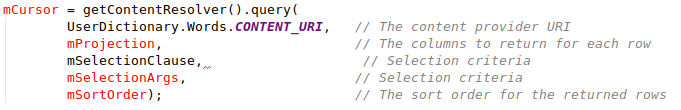
\includegraphics[width=\textwidth]{query}
	\begin{block}{}
		Zapytania powinny być wykonywane na innym wątku niż wątek UI, asynchronicznie. Jednym ze sposobów jest użycie klasy \textbf{CursorLoader}.
	\end{block}
	\begin{block}{}
		Aby móc pobierać dane z provider'a, aplikacja musi posiadać uprawnienia do odczytu z provider'a.
	\end{block}
\end{frame}

\begin{frame}{Argumenty query()}
	\centering
	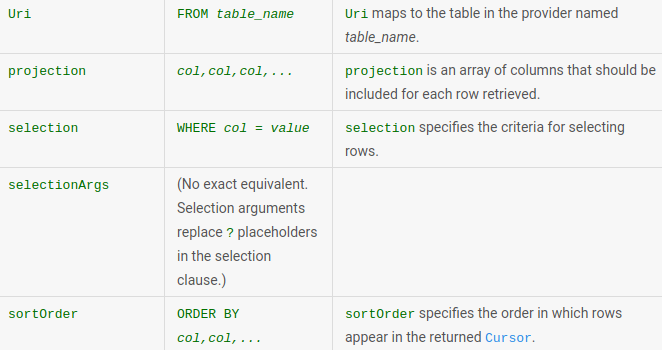
\includegraphics[width=0.9\textwidth]{query-args}
\end{frame}

\begin{frame}{Wyświetlanie rezultatów}
	\begin{block}{}
		Funkcja query zwraca zawsze obiekt klasy \textbf{Cursor}, który udostępnia losowy dostęp do wierszy i kolumn które zawiera. Dane te można następnie przekonwertować na ListView przy pomocy klasy \textbf{SimpleCursorAdapter}, lub użyć w innych miejscach (Cursor ma kilka metod get służących do pobierania różnych typów danych z obiektu).
	\end{block}
\end{frame}

\begin{frame}{Wstawianie danych}
	\centering
	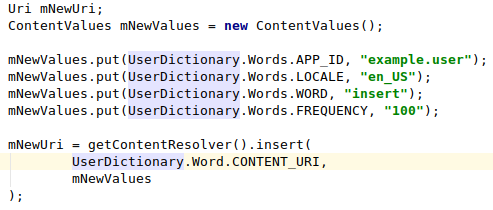
\includegraphics[width=0.8\textwidth]{insert}
	\begin{block}{}
		Dane dla nowego wiersza tworzymy przy pomocy klasy \textbf{ContentValues}, która reprezentuje pojedynczy wpis. Nie dodaje się kolumny ID, która jest dodawana automatycznie. Metoda insert zwraca content URI do wstawianego obiektu.
	\end{block}
\end{frame}

\begin{frame}{Aktualizacja danych}
	\begin{block}{}
		Do aktualizacji danych także używana jest klasa ContentValues, zawierająca tylko wartości, które chcemy zaktualizować. W metodzie update podawane są argumenty, które odpowiadają za wyszukanie wierszy, które mają zostać zaktualizowane. Metoda zwraca ilość zaktualizowanych wierszy.
	\end{block}
\end{frame}

\begin{frame}{Aktualizacja danych}
	\centering
	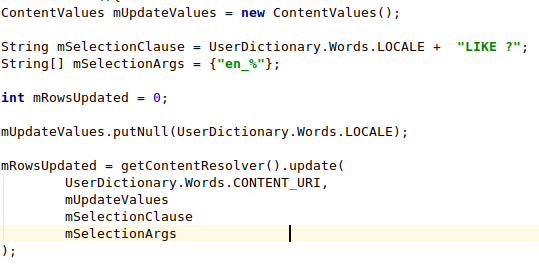
\includegraphics[width=0.8\textwidth]{update}
\end{frame}

\begin{frame}{Usuwanie danych}
	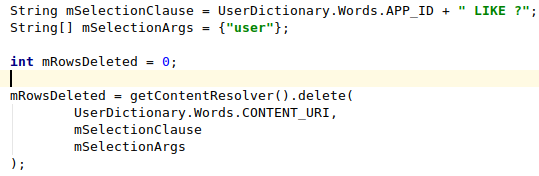
\includegraphics[width=0.8\textwidth]{delete}
	\begin{block}{}
		Do metody delete podajemy argumenty, które wyszukują wiersze, które chcemy usunąć. Metoda zwraca ilość usuniętych wierszy.
	\end{block}
\end{frame}

\begin{frame}{Tworzenie Content Provider'a}
	\begin{block}{}
		Tworzenie Content Provider'a polega na zaimplementowaniu metod klasy ContentProvider. Klasa ta definiuje 6 metod abstrakcyjnych które wymagają implementacji:
		\begin{itemize}
			\item query() - pobiera dane z provider'a, zwraca obiekt klasy Cursor
			\item insert() - wstawia dane do provider'a, zwraca Uri do wstawionego obiektu
			\item update() - aktualizuje wybrane wiersze, zwraca ilość zaktualizowanych wierszy
			\item delete() - usuwa wybrane wiersze, zwraca ilość usuniętych wierszy
			\item getType() - zwraca MIME type odpowiadający podanemu URI
			\item onCreate() - inicjalizuje provider
		\end{itemize}
	\end{block}
\end{frame}

\begin{frame}{Tworzenie Content Provider'a - kroki}
	\begin{enumerate}
		\item Stworzenie podklasy klasy ContentProvider
		\item Zdefiniowanie URI którym będzie posługiwał się Content Provider
		\item Stworzenie bazdy danych
		\item Implementacja różnych query wykonujących różne operacje na bazie danych
		\item Zarejestrowanie provider'a w manifeście poprzez użycie tagu \textbf{<provider>}
	\end{enumerate}
\end{frame}

\begin{frame}{Serwisy}
	\begin{block}{}
		Serwis jest komponentem aplikacji, który wykonuje długo trwające operacje (np: update do bazy danych, pobieranie pliku z sieci) oraz nie zapewnia UI(user interface).
		
		Serwisy są uruchamiane przez inne komponenty np: Activity. Dodatkowo serwis może zostać "związany" z komponentem który go uruchomił, w takim przypadku możemy wchodzić w interakcje z serwisem czyli wykonywać metody które się w nim znajdują.
	\end{block}
\end{frame}

\begin{frame}{Typy serwisów}
	\begin{itemize}
		\item \textbf{Foreground} - wykonuje operacje zauważalne dla użytkownika. Serwisy te działają nawet wtedy gdy użytkownik nie uzywa aplikacji
		\item \textbf{Background} - wykonuje operacje, o których użytkownik nie jest bezpośrednio informowany.
		\item \textbf{Bound} - Serwis jest związany gdy komponent aplikacji wiąże się z nim przy pomocy metody \textbf{bindService}. Komponent dostaje wtedy do dyspozycji prosty interface IBinder dzięki któremu może nawiązać komunikacje z serwisem.
	\end{itemize}
\end{frame}

\begin{frame}{Tworzenie serwisu}
	\begin{block}{}
		Aby stworzyć serwis, trzeba stworzyć podklasę klasy Service lub jednej z jej istniejących już podklas.
		Metody które należy przeciążyć podczas tworzenia serwisu:
		\begin{itemize}
			\item \textbf{onStartCommand()} - metoda wywoływana po wywołaniu startService. Po wykonaniu tej metody serwis jest wystartowany i może działać w tle przez czas nieokreślony. Jeśli przeciążymy tą metodę, to zatrzymanie serwisu trzeba takze zaimplementować poprzez wywołanie metod \textbf{stopSelf} lub \textbf{stopService}.
			\item \textbf{onBind()} - metoda wywoływana po wywołaniu bindService. Musi się tu znaleźć implementacja interfejsu którego klient będzie używać do komunikacji z serwisem.
		\end{itemize}
	\end{block}
\end{frame}

\begin{frame}{Tworzenie serwisu}
	\begin{block}{}
		\begin{itemize}
			\item \textbf{onCreate()}
			\item \textbf{onDestoy()}
		\end{itemize}
	\end{block}
\end{frame}

\begin{frame}{Dodanie serwisu do manifestu}
	\begin{block}{}
		Wszystkie serwisy muszą być zadeklarowane w manifeście aplikacji.
	\end{block}
	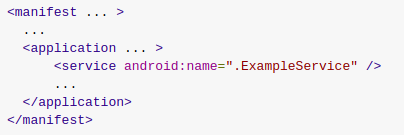
\includegraphics[width=0.8\textwidth]{service-manifest}
\end{frame}

\begin{frame}{Przykład implementacji started service}
	\centering
	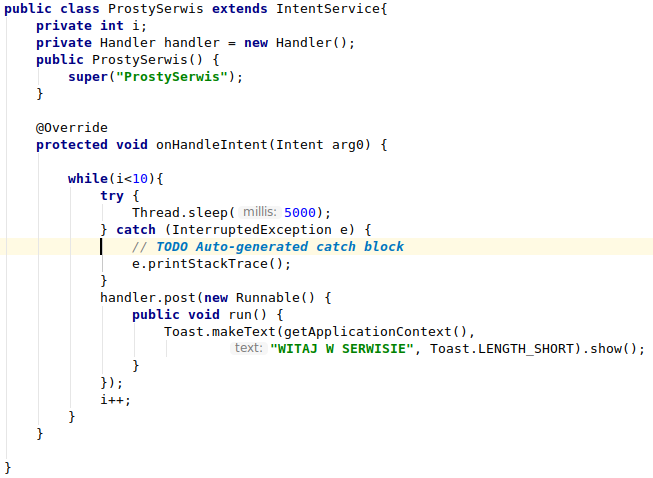
\includegraphics[height=0.8\textheight]{started-service}
\end{frame}

\begin{frame}{Przykład wystartowania started service}
	\begin{block}{}
		startService(new Intent(getBaseContext(), ProstySerwis.class));
	\end{block}
\end{frame}

\begin{frame}{Przykład implementacji bound service}
	\centering
	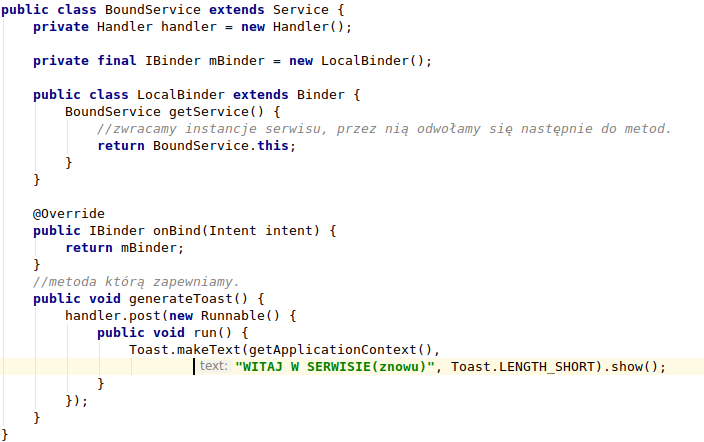
\includegraphics[height=0.8\textheight]{bound-service}
\end{frame}

\begin{frame}{Przykład połączenia z bound service}
	\begin{block}{}
		Intent intent = new Intent(this, BoundService.class);
		bindService(intent, mConnection, Context.BIND\_AUTO\_CREATE);
	\end{block}
\end{frame}

\end{document}

